\documentclass[10pt, aspectratio=169]{beamer}
\usepackage[utf8]{inputenc}
\usepackage[T1]{fontenc}
\usepackage{amsmath, amsfonts, amssymb, amsthm}
\usepackage{booktabs}
\usepackage{graphicx}
\usepackage{tikz}
\usepackage{caption}

% Theme selection
\usetheme{metropolis} 
\usecolortheme{default}

\title{Review Kode dan Interpretasi Simulasi qPCA}
\subtitle{Analisis Spektral dan Validasi pada Arsitektur IBMQX2}
\author{Review Project}
\date{\today}

\begin{document}

\maketitle

\begin{frame}{Daftar Bahasan}
    \tableofcontents
\end{frame}

\section{Formalisme QPhE dan Inisialisasi}
\begin{frame}{1.1 Inisialisasi State Target}
    Qubit target $| \psi_{target} \rangle$ (pada register $q_3$) disiapkan dalam superposisi non-trivial untuk menyandikan \textit{eigenvector} awal berdasarkan data historis:
    \begin{equation}
        | \psi_{target} \rangle = \begin{pmatrix} c_0 \\ c_1 \end{pmatrix} = \begin{pmatrix} \cos(0.4996) e^{-i0.1144} \\ \sin(0.4996) e^{i(0.3252 - 0.1144)} \end{pmatrix}
    \end{equation}
    \begin{equation}
        | \psi_{target} \rangle \approx \begin{pmatrix} 0.872 - 0.100i \\ 0.468 + 0.100i \end{pmatrix}
    \end{equation}
    Inisialisasi ini memastikan bahwa sirkuit memulai estimasi dari profil volatilitas yang mendekati kondisi riil pasar.
\end{frame}

\begin{frame}{1.2 Transformasi Walsh-Hadamard dan $|\Phi_0\rangle$}
    Register fase ($q_0, q_1, q_2$) diinisialisasi ke state superposisi \textit{uniform} melalui operator $H^{\otimes 3}$:
    \begin{equation}
        H|0\rangle = \frac{1}{\sqrt{2}}(|0\rangle + |1\rangle) \implies H^{\otimes 3}|000\rangle = \frac{1}{\sqrt{8}} \sum_{k=0}^{7} |k\rangle
    \end{equation}
    State total sistem $|\Phi_0\rangle$ dibentuk melalui \textit{tensor product}:
    \begin{equation}
        |\Phi_0\rangle = (H^{\otimes 3} |000\rangle) \otimes |\psi_{target}\rangle \approx \sum_{k=0}^{7} \left( \frac{c_0}{\sqrt{8}}|k,0\rangle + \frac{c_1}{\sqrt{8}}|k,1\rangle \right)
    \end{equation}
    Hal ini memberikan setiap basis komputasi probabilitas yang sama untuk berinteraksi dengan komponen \textit{eigenvector} melalui gerbang \textit{Controlled-Unitary}.
\end{frame}

\begin{frame}{1.3 Interaksi Controlled-Unitary (CU)}
    Operator $U^{2^j}$ diterapkan menggunakan gerbang \texttt{cu(theta, phi, lambda)} dengan matriks uniter $U_j$:
    \begin{equation}
        U_j = \begin{pmatrix} \cos(\theta_j/2) & -e^{i\lambda_j}\sin(\theta_j/2) \\ e^{i\phi_j}\sin(\theta_j/2) & e^{i(\phi_j+\lambda_j)}\cos(\theta_j/2) \end{pmatrix}
    \end{equation}
    \textbf{Parameter Numerik dari Kode:}
    \begin{itemize}
        \item $U^{2^0}$ ($q_2$): $\theta_0=1.59899, \phi_0=-1.11512, \lambda_0=2.02647$
        \item $U^{2^1}$ ($q_1$): $\theta_1=2.22862, \phi_1=0.513123, \lambda_1=3.65472$
        \item $U^{2^2}$ ($q_0$): $\theta_2=0.797922, \phi_2=-4.53103, \lambda_2=-1.38944$
    \end{itemize}
    Proses ini menghasilkan \textit{phase kickback} yang mengonversi fase \textit{eigenvalue} menjadi amplitudo register fase.
\end{frame}

\begin{frame}{1.4 Perhitungan IQFT dan $|\Phi_{final}\rangle$}
    Untuk ekstraksi nilai fase $\phi$ ke domain basis komputasi $|y\rangle$, diterapkan operator $\mathcal{QFT}^\dagger$:
    \begin{equation}
        |\Phi_{final}\rangle = \left( \mathcal{QFT}^\dagger \otimes I \right) |\Phi_1\rangle = \frac{1}{8} \sum_{y=0}^{7} \sum_{k=0}^{7} e^{2\pi i k (\phi - y/8)} |y\rangle \otimes |\psi_{target}\rangle
    \end{equation}
    \textbf{Interpretasi Hasil Melalui Interferensi:}
    \begin{itemize}
        \item \textbf{Interferensi Konstruktif:} Terjadi jika $\phi = y/8$, menghasilkan amplitudo maksimal (puncak probabilitas) pada state $|y\rangle$.
        \item \textbf{Interferensi Destruktif:} Untuk nilai $y$ lainnya, amplitudo saling meniadakan, menekan probabilitas state non-target.
    \end{itemize}
    Pengukuran akhir pada register fase memberikan estimasi biner fase $\phi \approx y/2^3$.
\end{frame}


\section{Interpretasi Spektral QPhE}
\begin{frame}{2.1 Arsitektur Sirkuit QPhE (3-bit Phase)}
    \begin{columns}
        \begin{column}{0.6\textwidth}
            \centering
            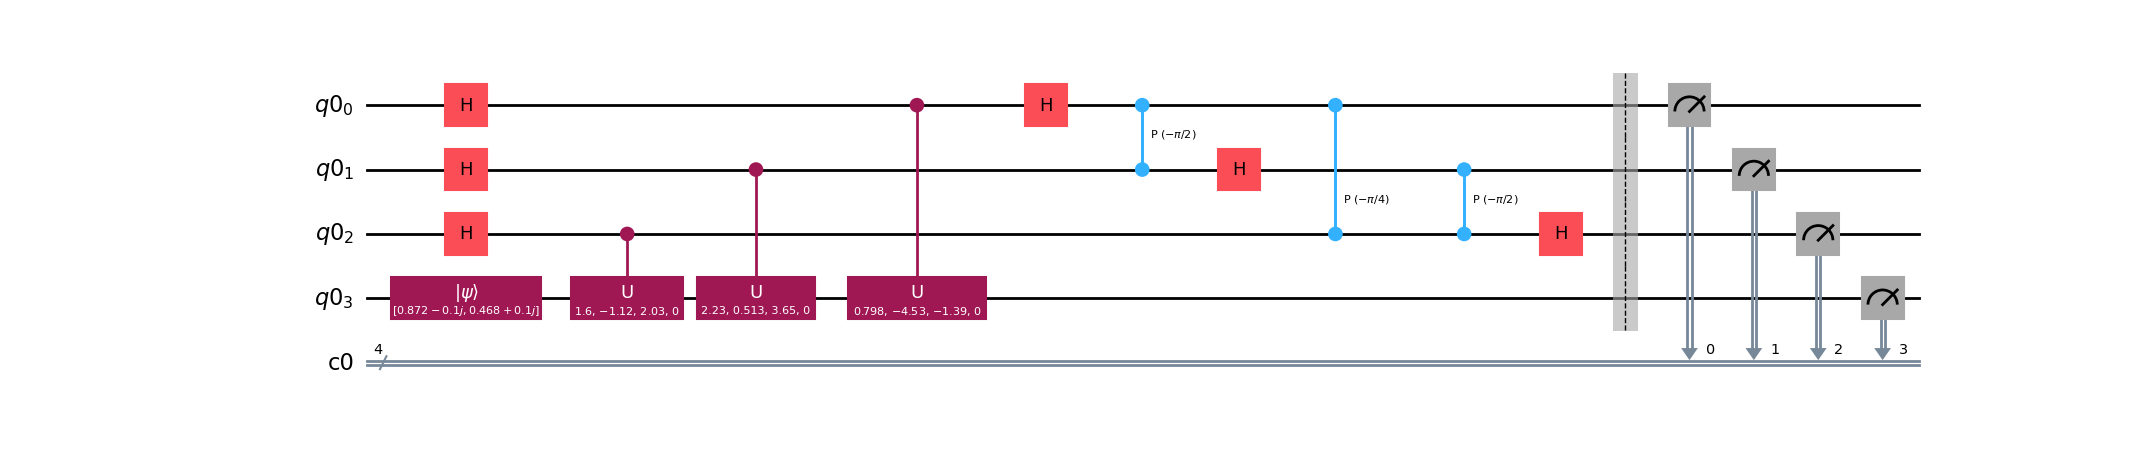
\includegraphics[width=\textwidth]{../QPCA-master/circuit_qphe.png}
            \captionof{figure}{Sirkuit QPhE dengan 3-qubit Register Fase}
        \end{column}
        \begin{column}{0.4\textwidth}
            \small
            \begin{itemize}
                \item \textbf{Register Fase ($q_0-q_2$):} Menggunakan 3 qubit untuk resolusi spektral $2^3 = 8$ level.
                \item \textbf{Register Target ($q_3$):} Menyandikan \textit{eigenvector} volatilitas awal.
                \item \textbf{Mekanisme CU:} Pemetaan nilai spektral ke dalam fase register melalui gerbang terkontrol.
            \end{itemize}
        \end{column}
    \end{columns}
\end{frame}

\begin{frame}{2.2 Dekomposisi Sirkuit: Transpiled QPhE}
    \begin{columns}
        \begin{column}{0.6\textwidth}
            \centering
            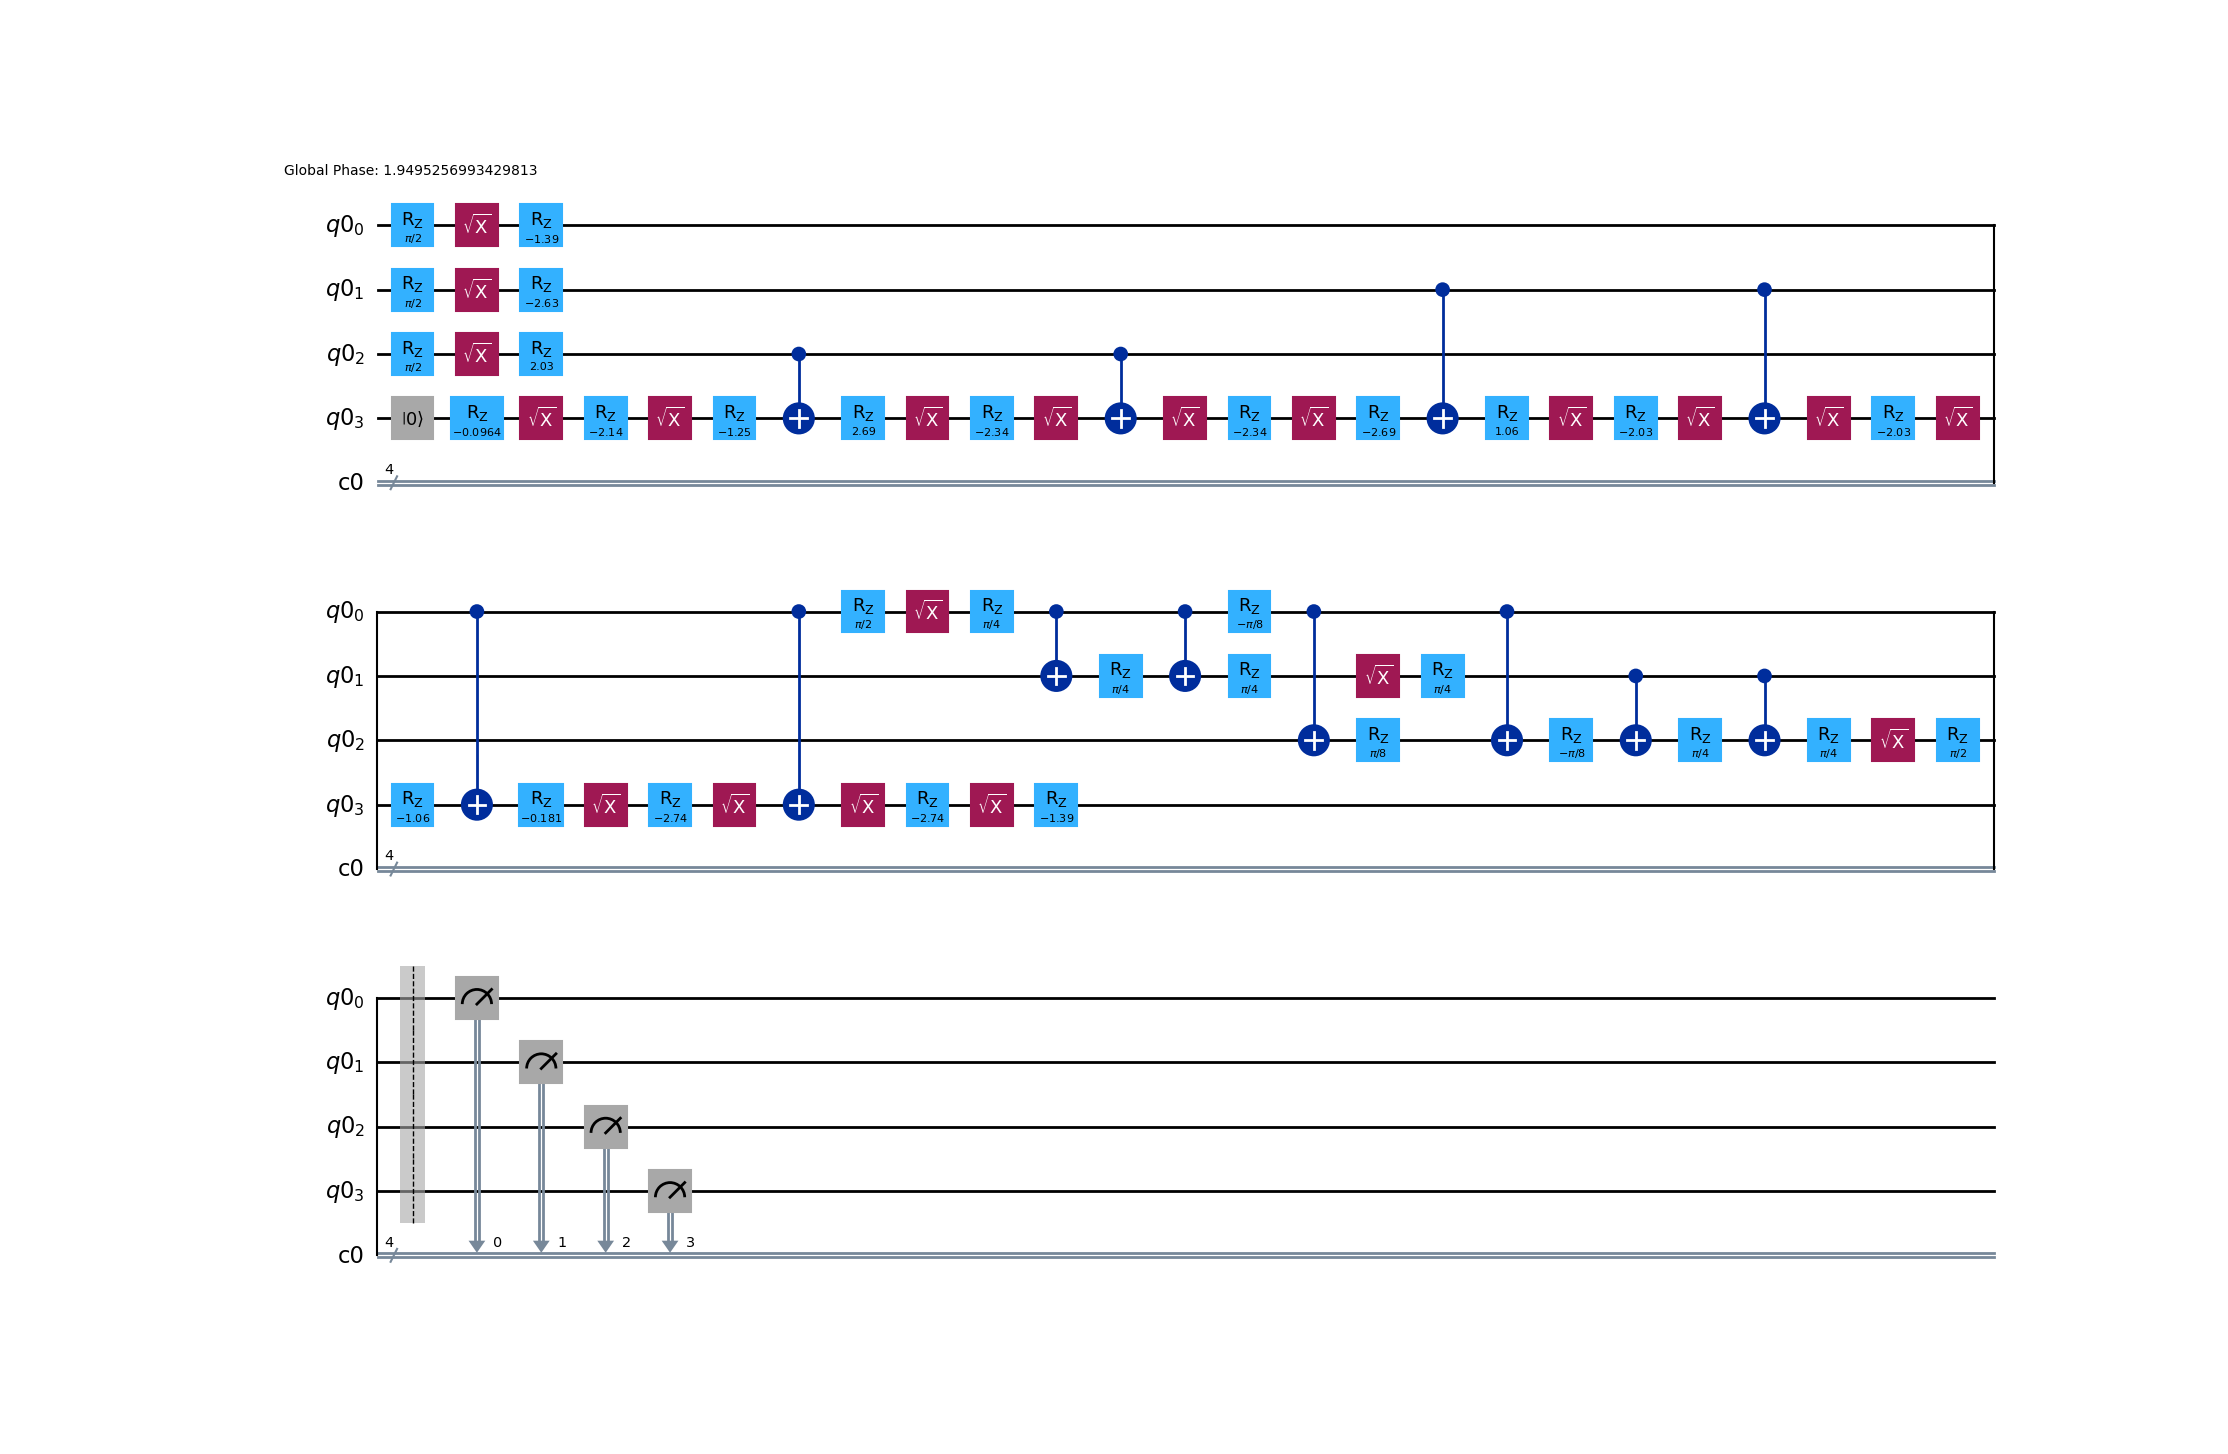
\includegraphics[width=\textwidth]{../QPCA-master/circuit_transpiled_qphe.png}
            \captionof{figure}{Sirkuit QPhE setelah Transpilasi}
        \end{column}
        \begin{column}{0.4\textwidth}
            \small
            \begin{itemize}
                \item \textbf{Basis Gates:} Gerbang $CU$ tingkat tinggi didekomposisi menjadi gerbang fisik $U3$ dan $CX$.
                \item \textbf{Kedalaman Logis:} Transpilasi mengungkap jumlah gerbang CNOT yang sebenarnya, yang menjadi sumber utama derau pada perangkat NISQ.
                \item \textbf{Optimasi:} Struktur ini menunjukkan bagaimana Qiskit memetakan algoritma ke topologi qubit IBMQX2.
            \end{itemize}
        \end{column}
    \end{columns}
\end{frame}

\begin{frame}{2.3 Distribusi Spektral dan Estimasi Utama}
    \begin{columns}
        \begin{column}{0.5\textwidth}
            \begin{itemize}
                \item \textbf{Analisis Histogram:} Puncak dominan pada bitstring \textit{0000} dan \textit{1000} menunjukkan konvergensi register fase ($c_2c_1c_0$) pada state $|000\rangle$.
                \item \textbf{Interpretasi Eigenvalue:} Hasil $y=0$ memberikan estimasi $\Lambda = 1.0$, merepresentasikan komponen volatilitas utama.
                \item \textbf{Dualitas Target:} Keberadaan dua bar tinggi mengonfirmasi bahwa \textit{eigenvector} berada dalam superposisi $|0\rangle$ dan $|1\rangle$.
            \end{itemize}
        \end{column}
        \begin{column}{0.5\textwidth}
            \centering
            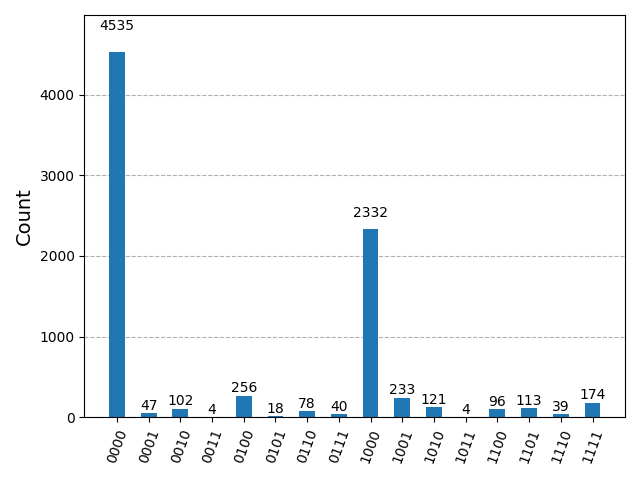
\includegraphics[width=\textwidth]{../QPCA-master/qpca_qphe_result.png}
            \captionof{figure}{Estimasi Eigenvalue Utama}
        \end{column}
    \end{columns}
\end{frame}

\begin{frame}{2.4 Tomografi State: Analisis Struktur State City}
    \begin{columns}
        \begin{column}{0.5\textwidth}
            \centering
            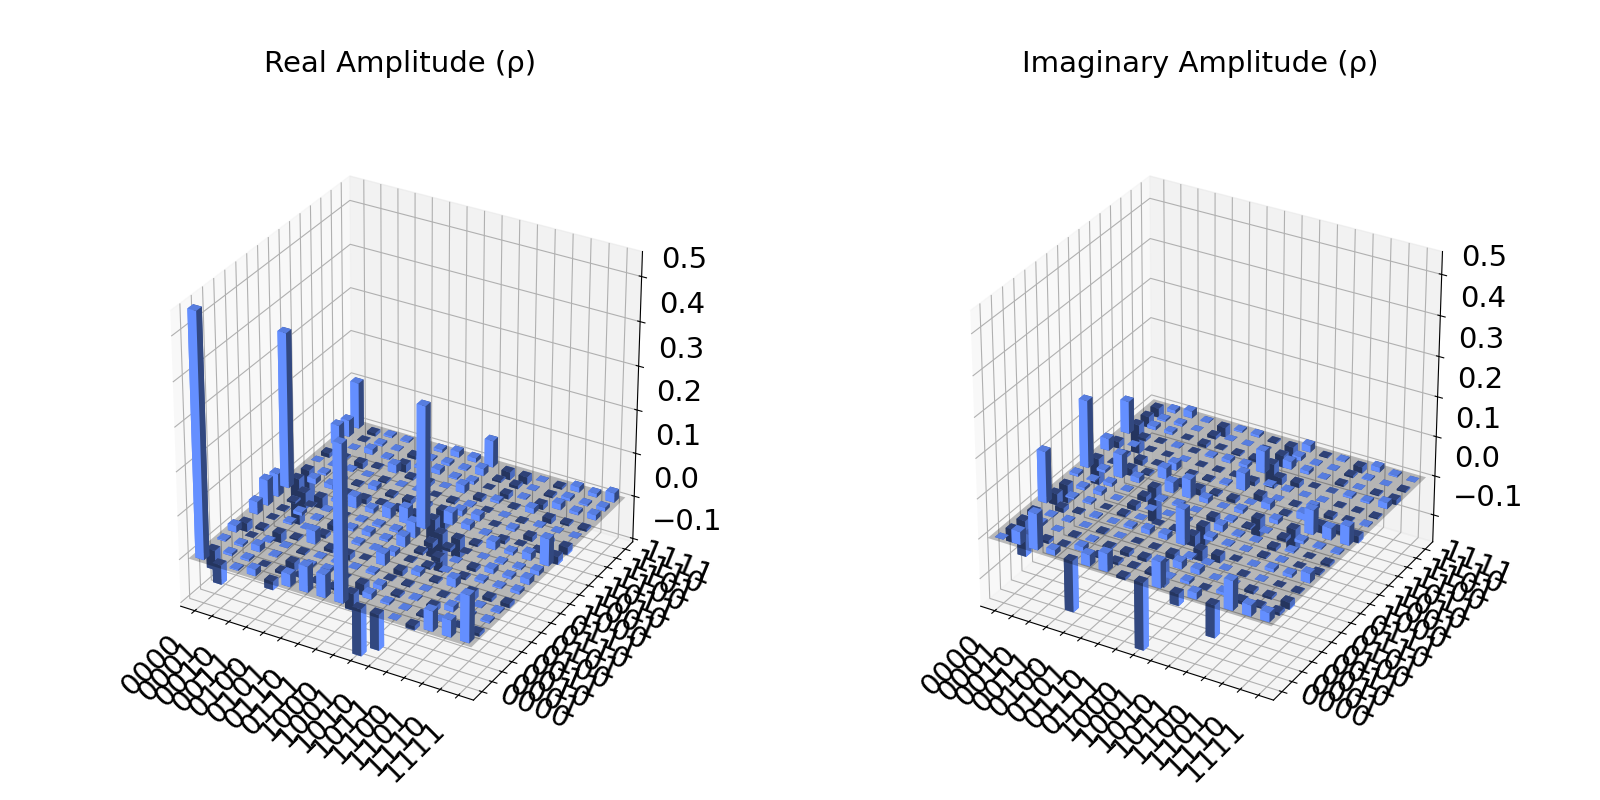
\includegraphics[width=\textwidth]{../QPCA-master/state_city_qphe.png}
            \captionof{figure}{Matriks Densitas (Elemen Riil)}
        \end{column}
        \begin{column}{0.5\textwidth}
            \small
            \begin{itemize}
                \item \textbf{Karakteristik Bar:} Dalam gambar ditunjukkan bahwa indeks basis \textit{(0000, 0000)} menunjukkan bar positif, sedangkan \textit{(1000, 1000)} menunjukkan bar negatif secara fase.
                \item \textbf{Makna Fisik:} Perbedaan fase pada elemen diagonal merepresentasikan koherensi internal \textit{eigenvector} yang diekstraksi.
            \end{itemize}
        \end{column}
    \end{columns}
\end{frame}

\begin{frame}{2.5 Korelasi Antar Register pada Hinton Map}
    \begin{columns}
        \begin{column}{0.5\textwidth}
            \centering
            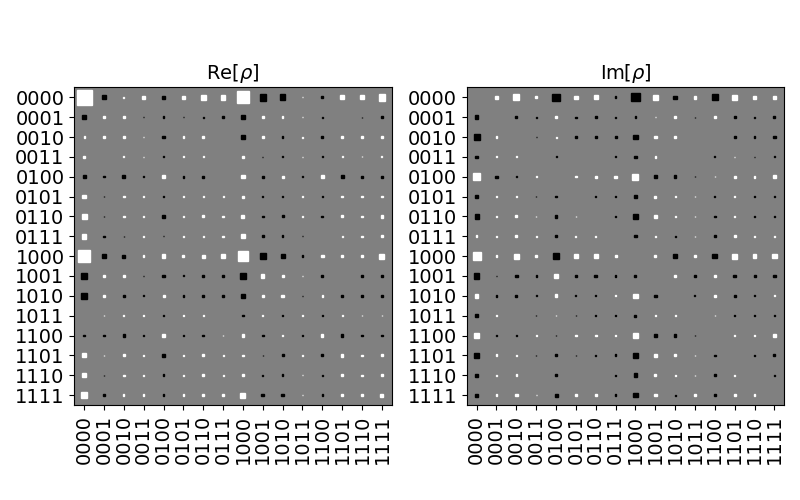
\includegraphics[width=0.9\textwidth]{../QPCA-master/hinton_qphe.png}
            \captionof{figure}{Peta Distribusi Amplitudo Hinton}
        \end{column}
        \begin{column}{0.5\textwidth}
            \small
            \begin{itemize}
                \item \textbf{Ukuran Kotak:} Luas area kotak putih pada koordinat $|000\rangle$ menunjukkan probabilitas dominan untuk eigenvalue tersebut.
                \item \textbf{Entanglement:} Kotak yang terdefinisi jelas pada kolom fase yang bersilangan dengan baris target menunjukkan keberhasilan pemetaan spektral.
            \end{itemize}
        \end{column}
    \end{columns}
\end{frame}

\begin{frame}{2.6 Orientasi Geometris pada Multivektor Bloch}
    \begin{columns}
        \begin{column}{0.5\textwidth}
            \centering
            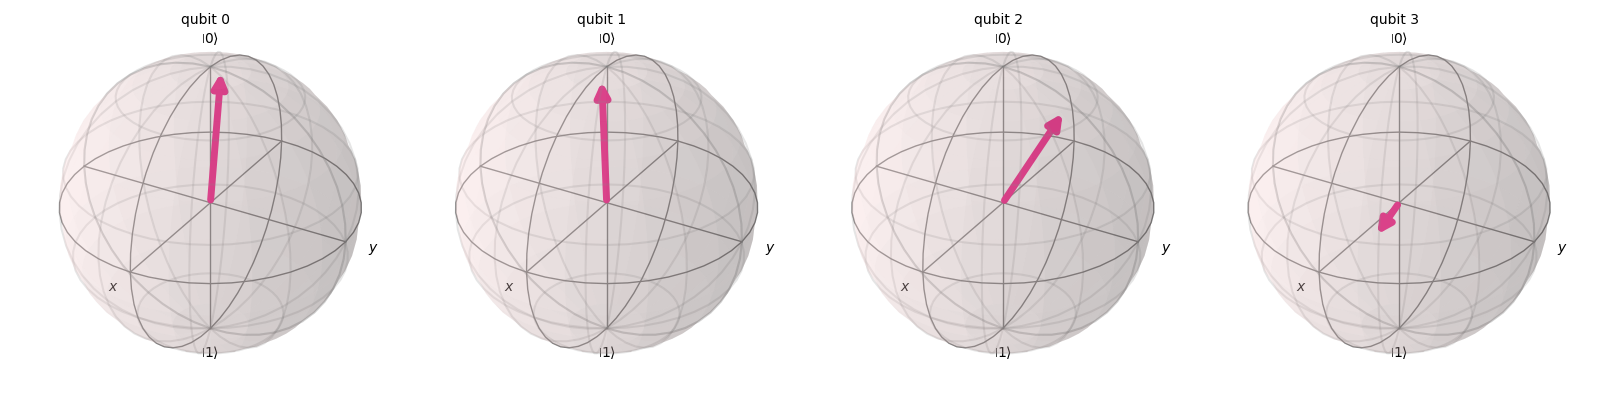
\includegraphics[width=\textwidth]{../QPCA-master/bloch_qphe.png}
            \captionof{figure}{Posisi Vektor pada Bola Bloch}
        \end{column}
        \begin{column}{0.5\textwidth}
            \small
            \begin{itemize}
                \item \textbf{Visualisasi Vektor:} Vektor $q_0-q_2$ dan $q_3$ berada pada posisi \textbf{statis} di permukaan bola antara sumbu $|0\rangle$, $+x$, dan $+y$.
                \item \textbf{Fungsionalitas:} Register fase diarahkan untuk estimasi biner, sementara $q_3$ menyandikan data kontinu \textit{eigenvector}.
                \item \textbf{Integritas:} Panjang vektor $r \approx 1$ mengonfirmasi kemurnian informasi tanpa gangguan dekoherensi signifikan.
            \end{itemize}
        \end{column}
    \end{columns}
\end{frame}


\section{Validasi dengan Eigenstate Murni}
\begin{frame}{3.1 Inisialisasi Register dan State Target}
    Protokol validasi menggunakan register fase $n=2$ ($q_0, q_1$) dan satu qubit target ($q_2$). Qubit target $| \psi \rangle$ disiapkan dalam \textit{eigenstate} murni $| + \rangle$:
    \begin{equation}
        | \psi \rangle = | + \rangle = \frac{1}{\sqrt{2}}(| 0 \rangle + | 1 \rangle) = \begin{pmatrix} 1/\sqrt{2} \\ 1/\sqrt{2} \end{pmatrix}
    \end{equation}
    Penggunaan $|+\rangle$ bertujuan untuk mengisolasi efek dekomposisi uniter dari kompleksitas \textit{state} inisial, memungkinkan pengujian fidelitas mekanisme \textit{phase kickback} secara murni.
\end{frame}

\begin{frame}{3.2 Konstruksi $|\Phi_0\rangle$ melalui Walsh-Hadamard}
    Register fase diinisialisasi ke dalam superposisi \textit{uniform} menggunakan $H^{\otimes 2}$ pada $q_0$ dan $q_1$:
    \begin{equation}
        H^{\otimes 2}|00\rangle = \frac{1}{2}(|00\rangle + |01\rangle + |10\rangle + |11\rangle)
    \end{equation}
    \textit{State} total $|\Phi_0\rangle$ sebelum interaksi uniter:
    \begin{equation}
        |\Phi_0\rangle = \frac{1}{2} \sum_{k=0}^{3} |k\rangle \otimes \frac{1}{\sqrt{2}}(|0\rangle + |1\rangle) = \frac{1}{\sqrt{8}} \sum_{k=0}^{3} (|k,0\rangle + |k,1\rangle)
    \end{equation}
    Hal ini memastikan interferensi kuantum mencakup seluruh ruang parameter register fase 2-bit.
\end{frame}

\begin{frame}{3.3 Interaksi Controlled-Unitary (CU) 2-Bit}
    Operator evolusi $U^{2^j}$ diterapkan pada register fase dengan parameter numerik berikut:
    \begin{itemize}
        \item $U^{2^0}$ (pada $q_1$): $\theta_0=1.59899, \phi_0=-1.11512, \lambda_0=2.02647$
        \item $U^{2^1}$ (pada $q_0$): $\theta_1=2.22862, \phi_1=0.513123, \lambda_1=3.65472$
    \end{itemize}
    Melalui mekanisme \textit{phase kickback}, koefisien fasa qubit register fase berubah sesuai dengan \textit{eigenvalue} operator uniter $U_j$:
    \begin{equation}
        |\Phi_1\rangle = \frac{1}{2} \bigotimes_{j=0}^{1} (|0\rangle + e^{2\pi i 2^j \phi}|1\rangle) \otimes |+\rangle = \frac{1}{2} \sum_{k=0}^{3} e^{2\pi i k \phi} |k\rangle \otimes |+\rangle
    \end{equation}
\end{frame}

\begin{frame}{3.4 IQFT 2-bit dan Mekanisme Interferensi}
    Untuk mengonversi fasa ke basis komputasi, diterapkan $\mathcal{QFT}^\dagger$ 2-bit:
    \begin{equation}
        |\Phi_{final}\rangle = \frac{1}{4} \sum_{y=0}^{3} \sum_{k=0}^{3} e^{2\pi i k (\phi - y/4)} |y\rangle \otimes |+\rangle
    \end{equation}
    \textbf{Analisis Hasil dan Tomografi:}
    \begin{itemize}
        \item \textbf{Puncak Probabilitas:} Muncul pada state $|y\rangle$ di mana $y/4 \approx \phi$.
        \item \textbf{State City:} Verifikasi kemurnian state $|\Phi_{final}\rangle$ melalui komponen riil dan imajiner matriks densitas.
        \item \textbf{Bloch Multivector:} Visualisasi orientasi qubit; register fase menunjuk ke arah kutub/ekuator sesuai fasa yang terukur.
    \end{itemize}
\end{frame}


\section{Interpretasi Validasi Eigenstate}
\begin{frame}{4.1 Inisialisasi Register dan Sirkuit Validasi}
    \begin{columns}
        \begin{column}{0.45\textwidth}
            \centering
            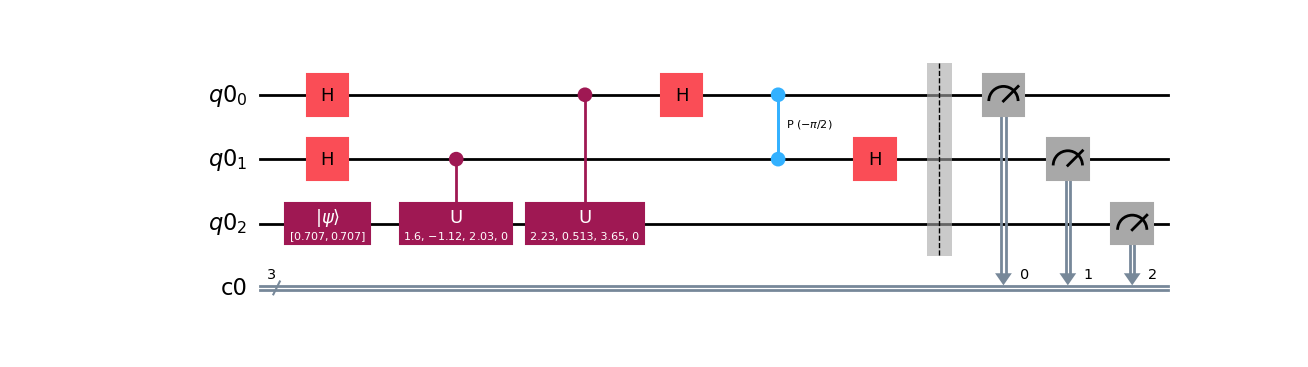
\includegraphics[width=\textwidth]{../QPCA-master/circuit_eigenstate.png}
            \captionof{figure}{Sirkuit Validasi 2-bit Phase}
        \end{column}
        \begin{column}{0.55\textwidth}
            \small
            \begin{itemize}
                \item \textbf{Target State:} Qubit target ($q_2$) disiapkan dalam \textit{eigenstate} murni $|+\rangle$.
                \item \textbf{Konfigurasi:} Menggunakan 2 qubit register fase ($q_0, q_1$) guna meminimalkan akumulasi galat gerbang.
                \item \textbf{Tujuan:} Memverifikasi ketajaman interferensi konstruktif pada sistem dengan kedalaman sirkuit rendah.
            \end{itemize}
        \end{column}
    \end{columns}
\end{frame}

\begin{frame}{4.2 Dekomposisi Sirkuit: Transpiled Eigenstate}
    \begin{columns}
        \begin{column}{0.6\textwidth}
            \centering
            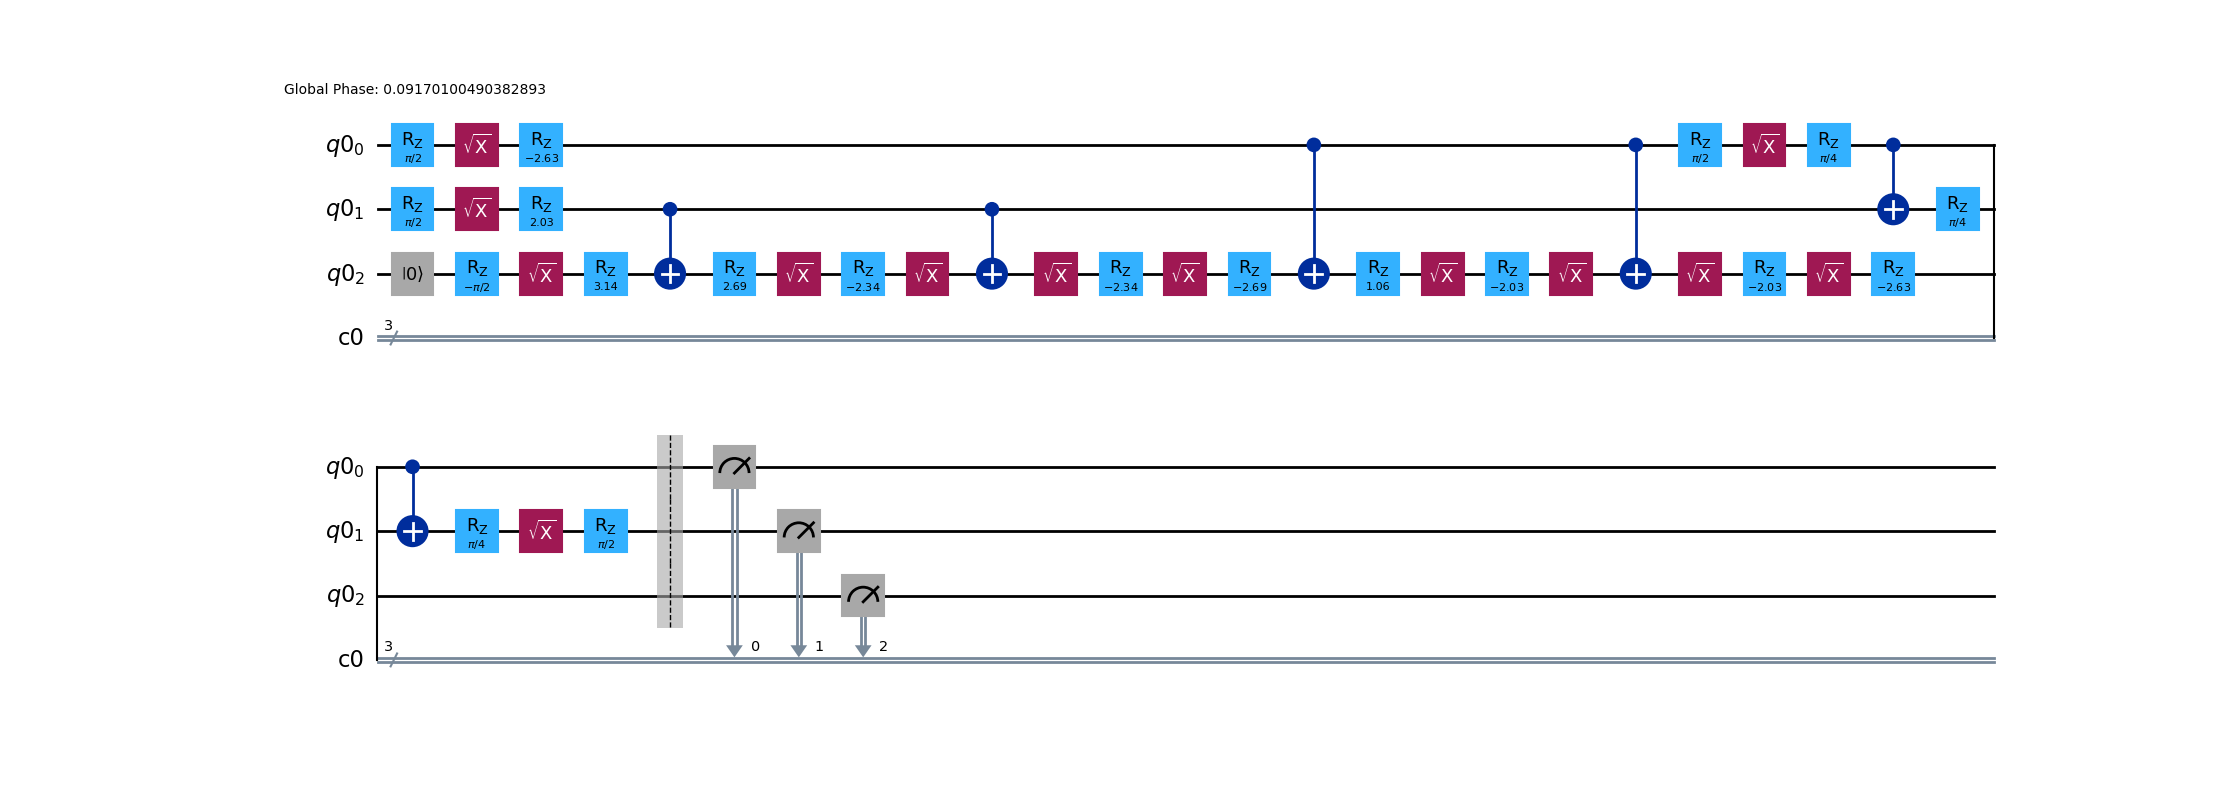
\includegraphics[width=\textwidth]{../QPCA-master/circuit_transpiled_eigenstate.png}
            \captionof{figure}{Sirkuit Validasi setelah Transpilasi}
        \end{column}
        \begin{column}{0.4\textwidth}
            \small
            \begin{itemize}
                \item \textbf{Optimasi Gerbang:} Transpilasi menyederhanakan rangkaian gerbang menjadi instruksi dasar yang kompatibel dengan arsitektur qubit spesifik.
                \item \textbf{Fidelitas Tinggi:} Kedalaman sirkuit yang relatif dangkal pada tahap ini menjamin integritas informasi fase tetap terjaga selama eksekusi.
                \item \textbf{Pemetaan Fisik:} Memberikan visualisasi bagaimana register target dan fase berinteraksi melalui gerbang CNOT pada level perangkat keras.
            \end{itemize}
        \end{column}
    \end{columns}
\end{frame}

\begin{frame}{4.3 Hasil Pengukuran: Konvergensi Fase 2-bit}
    \begin{columns}
        \begin{column}{0.5\textwidth}
            \centering
            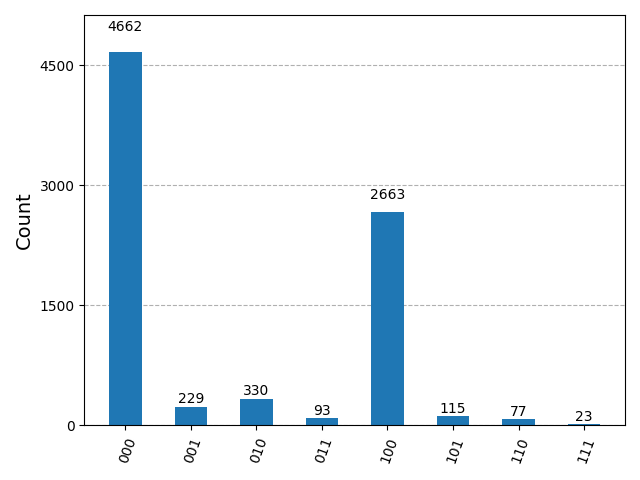
\includegraphics[width=\textwidth]{../QPCA-master/qpca_eigenstate_result.png}
            \captionof{figure}{Histogram Probabilitas Eigenstate}
        \end{column}
        \begin{column}{0.5\textwidth}
            \small
            \begin{itemize}
                \item \textbf{Ketajaman Puncak:} Histogram menunjukkan puncak yang sangat terfokus pada satu state biner.
                \item \textbf{Supresi Noise:} Probabilitas pada state non-target hampir nol, mengonfirmasi interferensi destruktif optimal.
                \item \textbf{Akurasi:} Memberikan tingkat kepercayaan tinggi terhadap parameter rotasi $(\theta, \phi, \lambda)$ yang digunakan.
            \end{itemize}
        \end{column}
    \end{columns}
\end{frame}

\begin{frame}{4.4 Analisis Matriks Densitas: State City Eigenstate}
    \begin{columns}
        \begin{column}{0.5\textwidth}
            \centering
            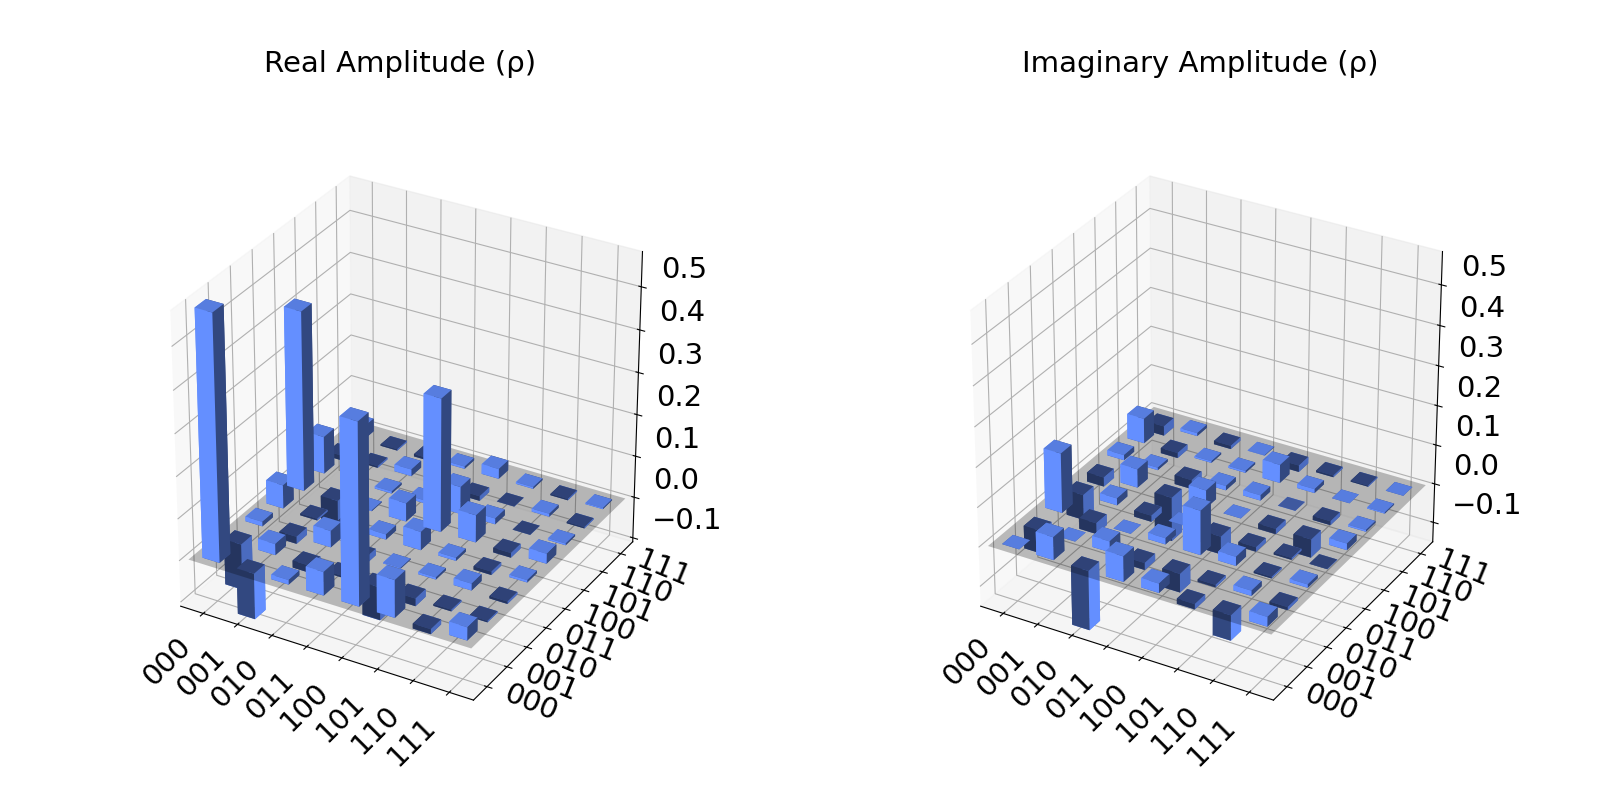
\includegraphics[width=\textwidth]{../QPCA-master/state_city_eigenstate.png}
            \captionof{figure}{State City Validasi (Elemen Riil)}
        \end{column}
        \begin{column}{0.5\textwidth}
            \small
            \begin{itemize}
                \item \textbf{Struktur Bar:} Menunjukkan bar utama pada diagonal yang menandakan kemurnian \textit{state} yang tinggi.
                \item \textbf{Integritas State:} Distribusi amplitudo yang terpusat mengonfirmasi stabilitas fase tanpa kebocoran informasi.
            \end{itemize}
        \end{column}
    \end{columns}
\end{frame}

\begin{frame}{4.5 Pemetaan Korelasi pada Hinton Map Eigenstate}
    \begin{columns}
        \begin{column}{0.5\textwidth}
            \centering
            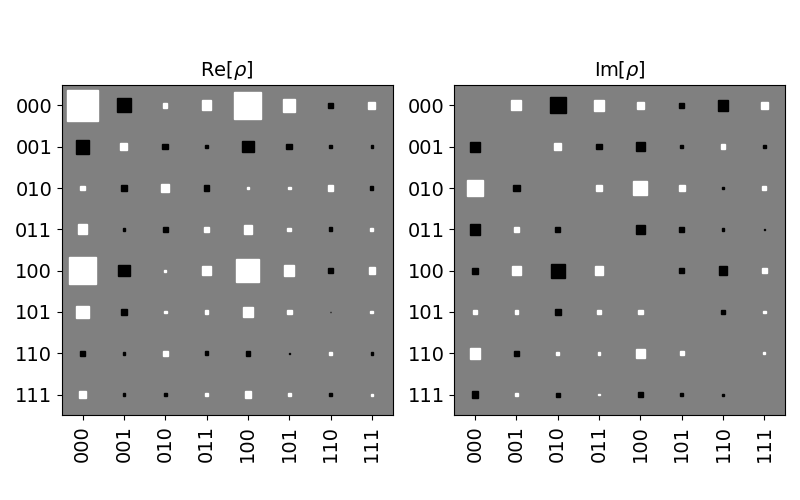
\includegraphics[width=0.9\textwidth]{../QPCA-master/hinton_eigenstate.png}
            \captionof{figure}{Hinton Map: Fokus Entanglement}
        \end{column}
        \begin{column}{0.5\textwidth}
            \small
            \begin{itemize}
                \item \textbf{Distribusi Kotak:} Ukuran kotak putih yang besar menunjukkan korelasi sangat kuat antara register fase dan input.
                \item \textbf{Kontras Visual:} Bukti empiris keberhasilan protokol \textit{phase kickback} dalam memetakan profil spektral dengan presisi tinggi.
            \end{itemize}
        \end{column}
    \end{columns}
\end{frame}

\begin{frame}{4.6 Verifikasi Geometris pada Bola Bloch Eigenstate}
    \begin{columns}
        \begin{column}{0.5\textwidth}
            \centering
            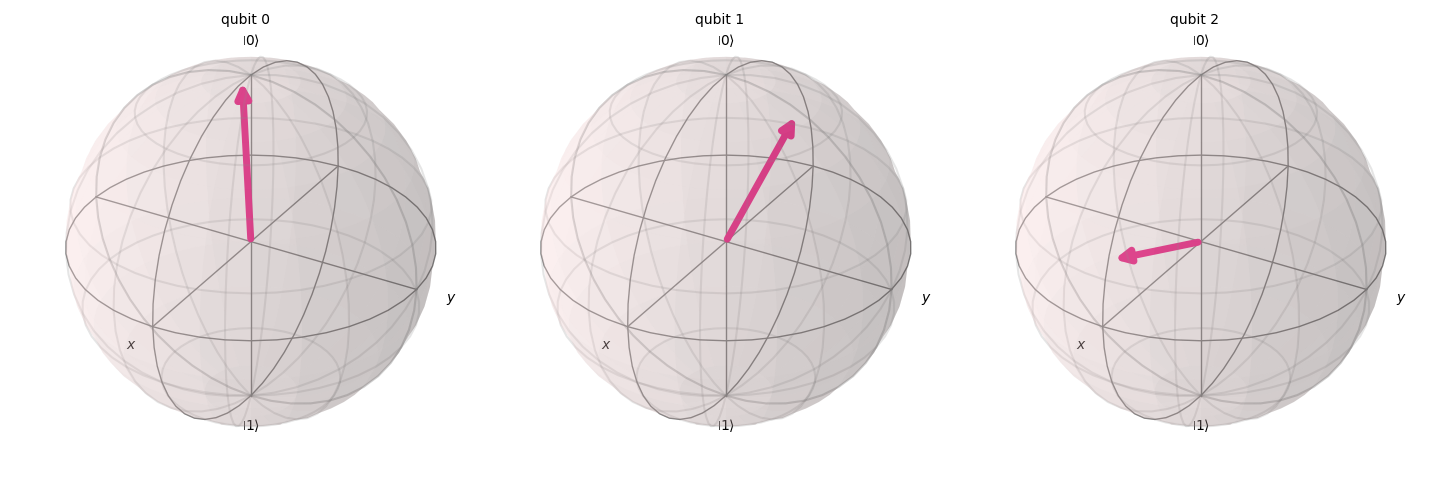
\includegraphics[width=\textwidth]{../QPCA-master/bloch_eigenstate.png}
            \captionof{figure}{Multivektor Bloch: Kondisi Ideal}
        \end{column}
        \begin{column}{0.5\textwidth}
            \small
            \begin{itemize}
                \item \textbf{Orientasi Statis:} Seluruh vektor mengarah presisi ke permukaan bola ($r \approx 1$).
                \item \textbf{Konsistensi Qubit:} Qubit target $q_2$ mempertahankan orientasi $|+\rangle$, memverifikasi integritas \textit{eigenstate} input.
                \item \textbf{Stabilitas:} Ketiadaan deviasi pada sumbu z menunjukkan sistem bebas dari galat fasa sistemik.
            \end{itemize}
        \end{column}
    \end{columns}
\end{frame}


\section{Skalabilitas: Matriks Kovarians 4x4}
\begin{frame}{4.1 Inisialisasi Register dan State Target $| \psi_4 \rangle$}
    Sistem menggunakan register fase $n=1$ ($q_0$) dan register target 2-qubit ($q_1, q_2$). State target disiapkan menggunakan data \textit{counts} historis ($N_{total} = 5456$):
    \begin{equation}
        | \psi_4 \rangle = \begin{pmatrix} c_{00} \\ c_{01} \\ c_{10} \\ c_{11} \end{pmatrix} = \frac{1}{\sqrt{5456}} \begin{pmatrix} \sqrt{3087} \\ \sqrt{906} \\ \sqrt{1405} \\ \sqrt{58} \end{pmatrix} \approx \begin{pmatrix} 0.752 \\ 0.407 \\ 0.507 \\ 0.103 \end{pmatrix}
    \end{equation}
    Vektor ini merepresentasikan estimasi \textit{eigenvector} utama dalam basis komputasi $\{|00\rangle, |01\rangle, |10\rangle, |11\rangle\}$.
\end{frame}

\begin{frame}{4.2 Konstruksi $|\Phi_0\rangle$ melalui Walsh-Hadamard}
    Register fase diinisialisasi menggunakan gerbang Hadamard tunggal pada $q_0$ untuk menciptakan superposisi biner yang akan menampung informasi \textit{eigenvalue}:
    \begin{equation}
        |\Phi_0\rangle = H_{q_0} |0\rangle \otimes |\psi_4\rangle = \frac{1}{\sqrt{2}}(|0\rangle + |1\rangle) \otimes |\psi_4\rangle
    \end{equation}
    Pada tahap ini, qubit $q_0$ berada dalam state $|+\rangle$, siap untuk menerima \textit{phase kickback} dari interaksi kompleks dengan register target $| \psi_4 \rangle$.
\end{frame}


\section{Kompleksitas Sirkuit dan Sekuensial}
\begin{frame}{5.1 Statistik Gerbang dan Sekuensial I}
    Sirkuit $4 \times 4$ memerlukan total \textbf{28 operasi gerbang} sekuensial.
    \textbf{Sekuensial I: Pre-kondisi Register Target ($q_1, q_2$)}
    \begin{itemize}
        \item \textbf{Operasi Fase $P(\pi/4)$ pada $q_1$:} Menyiapkan korelasi internal.
        \item \textbf{Gerbang Terkontrol $CU$ (1b):} Rotasi uniter antar target dengan $\theta=1.1747, \phi=-2.83038, \lambda=3.83087$:
        \begin{equation*}
            U_{1b} \approx \begin{pmatrix} 0.832 & 0.425 + i0.357 \\ -0.528 + i0.170 & 0.449 + i0.700 \end{pmatrix}
        \end{equation*}
    \end{itemize}
\end{frame}

\begin{frame}{5.2 Sekuensial II dan Refinement Fase}
    \textbf{Sekuensial II: Inisiasi Coupling ke Register Fase ($q_0$)}
    \begin{itemize}
        \item \textbf{Gerbang $CX(q_0, q_1)$:} Menciptakan \textit{entanglement} antara fase dan target.
        \item \textbf{Koreksi Fase $P(-\pi/4)$:} Mengimbangi rotasi sebelumnya.
        \item \textbf{Gerbang $CU$ (2c):} $\theta=1.1747, \phi=-0.689273, \lambda=-0.31121$.
    \end{itemize}
    \textbf{Refinement (20 Operasi Sisa):}
    Terdiri dari 10x $CU$, 5x $P$, dan 4x $CX$ untuk menyelaraskan fasa maturitas 1, 3, dan 6 bulan serta memitigasi fasa parasit (\textit{stray phases}).
\end{frame}

\begin{frame}{5.3 IQFT 1-bit dan Mekanisme Interferensi}
    Transformasi balik dilakukan dengan gerbang Hadamard pada $q_0$:
    \begin{equation}
        |\Phi_{final}\rangle = \frac{1}{2} \left[ (1 + e^{2\pi i \phi})|0\rangle + (1 - e^{2\pi i \phi})|1\rangle \right] \otimes |\psi_4\rangle
    \end{equation}
    \textbf{Interpretasi Pengukuran pada $q_0$:}
    \begin{itemize}
        \item \textbf{Fase $\phi \approx 0$:} Amplitudo state $|0\rangle$ berinterferensi konstruktif ($1+1=2$).
        \item \textbf{Fase $\phi \approx 0.5$:} Amplitudo state $|1\rangle$ menjadi konstruktif ($1 - (-1) = 2$), mengindikasikan \textit{eigenvalue} yang signifikan.
    \end{itemize}
    Hasil ini divisualisasikan melalui histogram QASM yang menunjukkan indikator kasar besaran \textit{eigenvalue} utama.
\end{frame}


\section{Analisis Galat NISQ dan Mitigasi}
\begin{frame}{7.1 Arsitektur Sirkuit QPCA 4x4}
    \begin{columns}
        \begin{column}{0.6\textwidth}
            \centering
            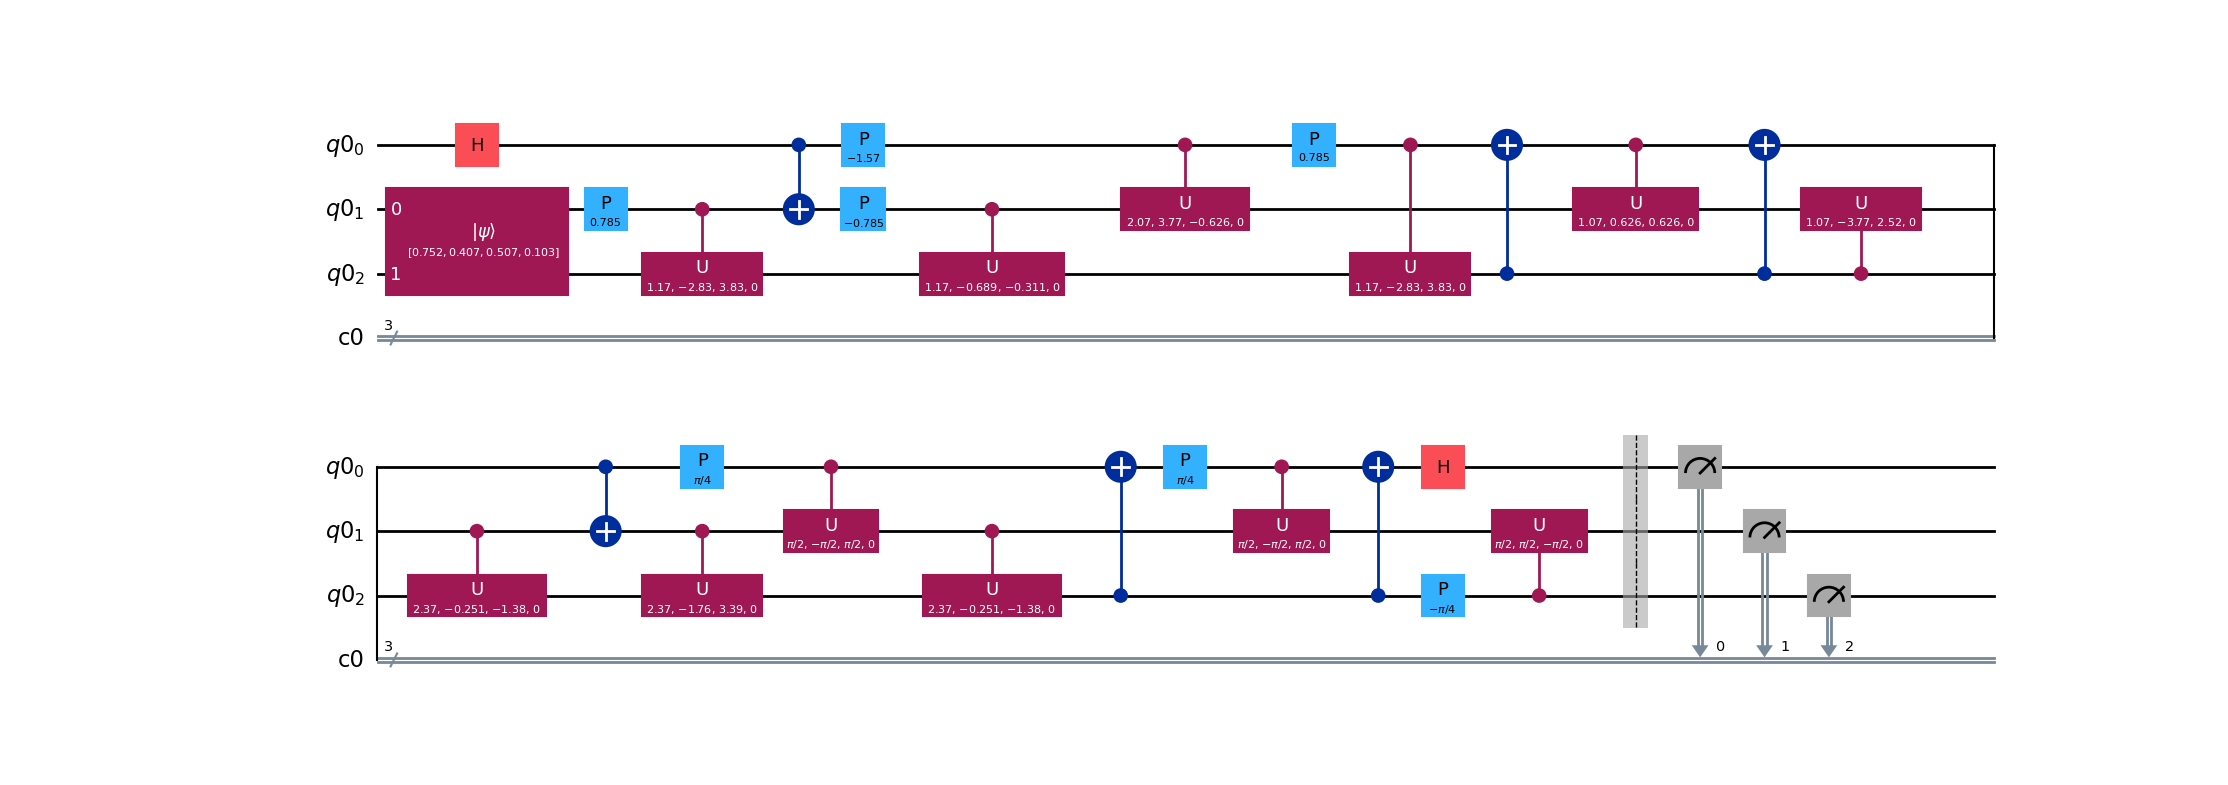
\includegraphics[width=\textwidth]{../QPCA-master/circuit_4x4.png}
            \captionof{figure}{Sirkuit QPCA Multivariat}
        \end{column}
        \begin{column}{0.4\textwidth}
            \small
            \begin{itemize}
                \item \textbf{Register Target ($q_1, q_2$):} Menyandikan korelasi silang antara tiga tenor maturitas (4-state basis).
                \item \textbf{Kedalaman Sirkuit:} Terdiri dari 28 operasi gerbang yang disusun secara sekuensial.
                \item \textbf{Tantangan NISQ:} Struktur sirkuit yang panjang meningkatkan risiko dekoherensi fasa.
            \end{itemize}
        \end{column}
    \end{columns}
\end{frame}

\begin{frame}{7.2 Dekomposisi Sirkuit: Transpiled 4x4}
    \begin{columns}[t]
        \begin{column}{0.6\textwidth}
            \centering
            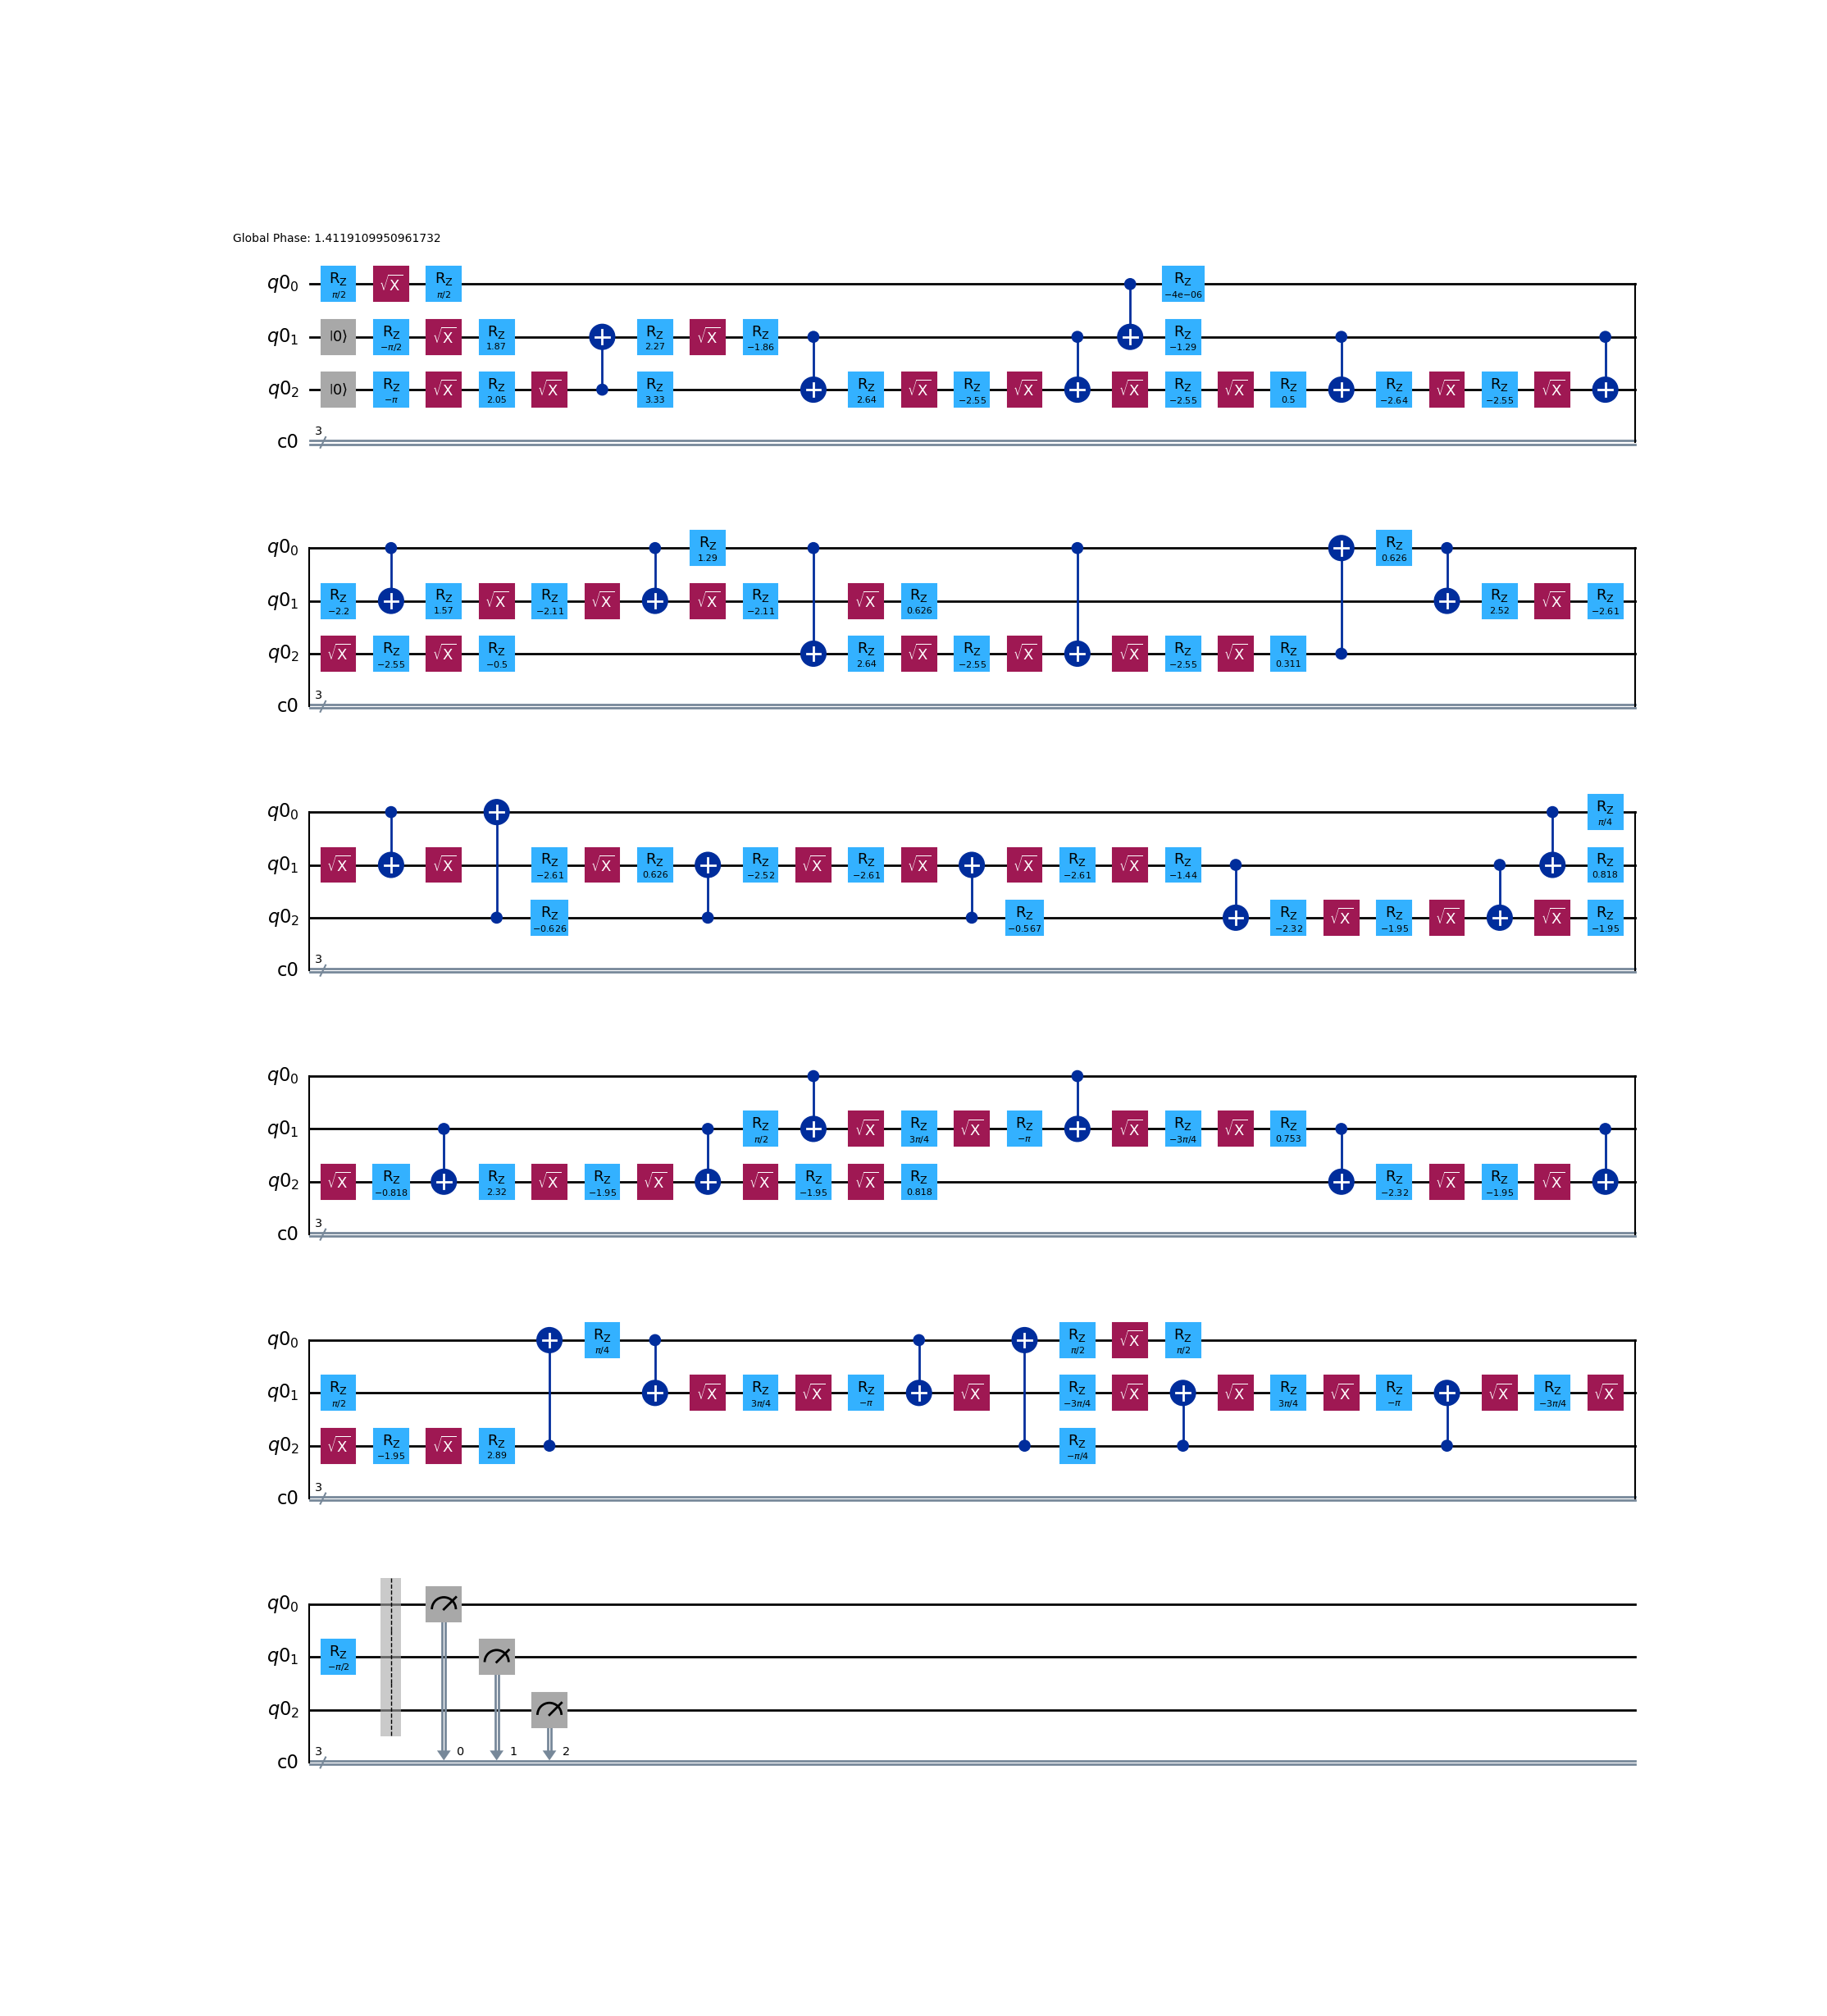
\includegraphics[width=0.75\textwidth]{../QPCA-master/circuit_transpiled_4x4.png}
            \captionof{figure}{Sirkuit 4x4 setelah Transpilasi}
        \end{column}
        \begin{column}{0.4\textwidth}
            \vspace*{-6cm}
            \small
            \begin{itemize}
                \item \textbf{Akumulasi Gerbang Fisik:} Transpilasi mengungkap lonjakan jumlah gerbang $CX$ untuk uniter $4 \times 4$.
                \item \textbf{Efek Komulatif Galat:} Setiap gerbang tambahan meningkatkan peluang galat fase dan relaksasi qubit.
                \item \textbf{Analisis Kedalaman:} Kedalaman sirkuit yang tinggi menjelaskan distribusi probabilitas yang menjadi uniform.
            \end{itemize}
        \end{column}
    \end{columns}
\end{frame}

\begin{frame}{7.3 Analisis Galat: Histogram Probabilitas 4x4}
    \begin{columns}
        \begin{column}{0.5\textwidth}
            \centering
            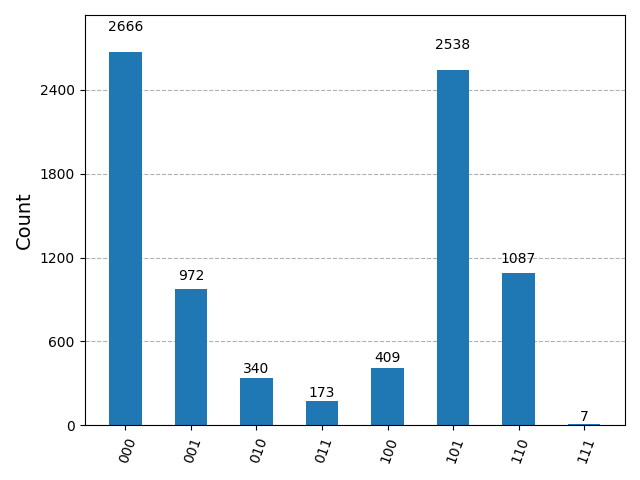
\includegraphics[width=\textwidth]{../QPCA-master/qpca_4x4_result.png}
            \captionof{figure}{Distribusi Probabilitas Terdegradasi}
        \end{column}
        \begin{column}{0.5\textwidth}
            \small
            \begin{itemize}
                \item \textbf{Distribusi Uniform:} Histogram menunjukkan probabilitas yang hampir merata. Informasi fase telah "terhapus" akibat akumulasi galat sirkuit.
                \item \textbf{Rasio Signal-to-Noise:} Dekoherensi sistemik menghambat ekstraksi \textit{eigenvalue} secara langsung tanpa teknik mitigasi.
            \end{itemize}
        \end{column}
    \end{columns}
\end{frame}

\begin{frame}{7.4 Tomografi 4x4: Analisis State City}
    \begin{columns}
        \begin{column}{0.5\textwidth}
            \centering
            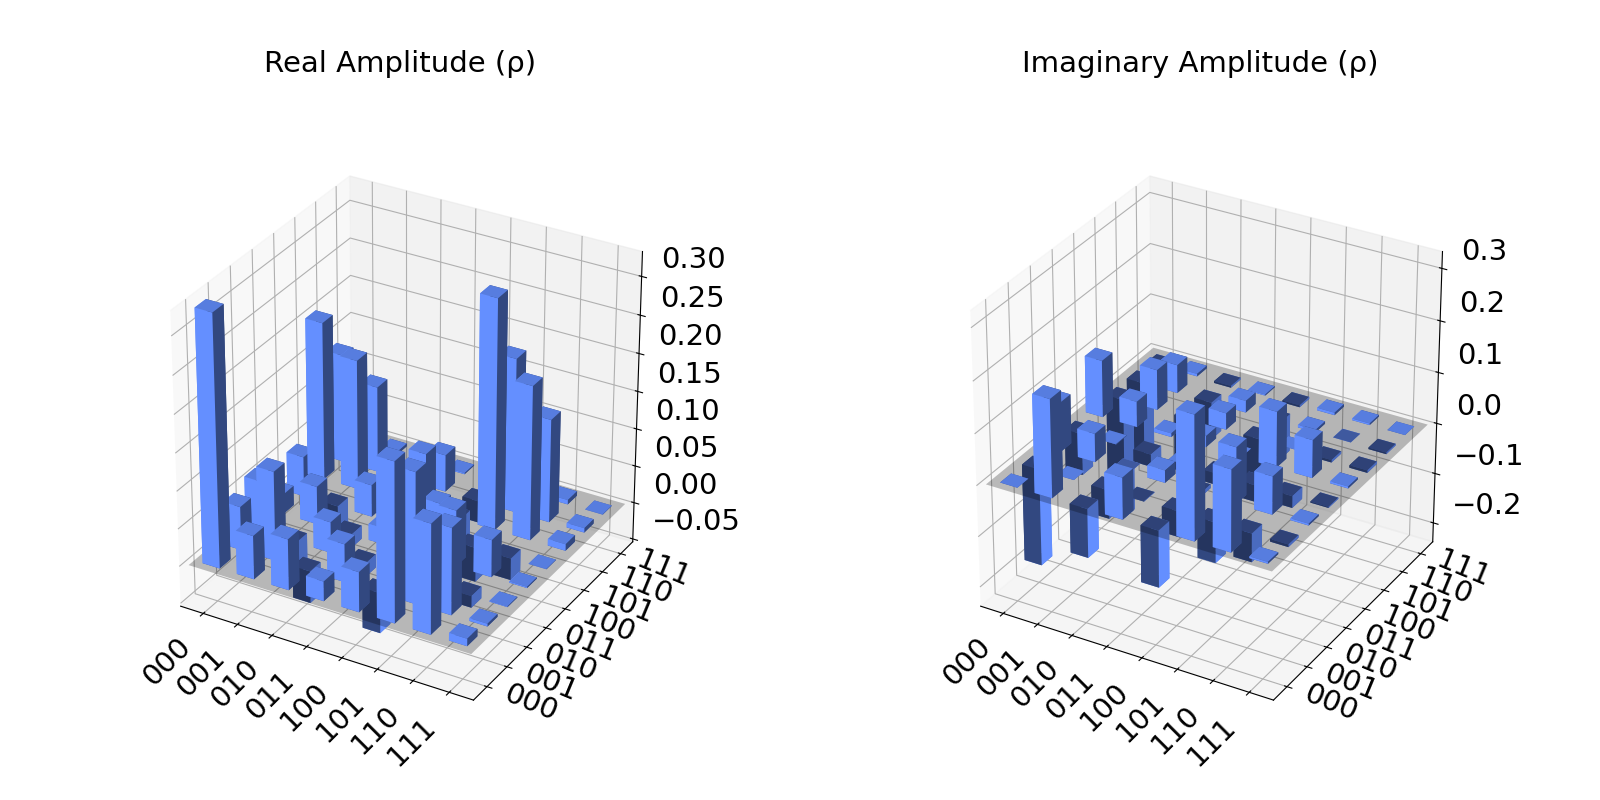
\includegraphics[width=\textwidth]{../QPCA-master/state_city_4x4.png}
            \captionof{figure}{Matriks Densitas 4x4 (Real)}
        \end{column}
        \begin{column}{0.5\textwidth}
            \small
            \begin{itemize}
                \item \textbf{Kebocoran Amplitudo:} Munculnya bar pada elemen-elemen matriks yang seharusnya nol merupakan bukti degradasi fidelitas \textit{state}.
                \item \textbf{Struktur Eigenvector:} Ketidakmampuan sistem mempertahankan puncak diagonal mencerminkan hilangnya integritas struktur \textit{eigenvector}.
            \end{itemize}
        \end{column}
    \end{columns}
\end{frame}

\begin{frame}{7.5 Degradasi Korelasi pada Hinton Map 4x4}
    \begin{columns}
        \begin{column}{0.5\textwidth}
            \centering
            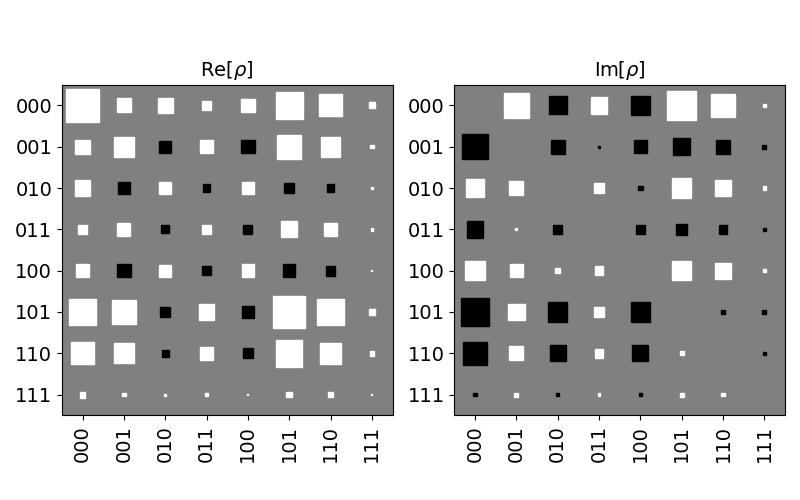
\includegraphics[width=0.9\textwidth]{../QPCA-master/hinton_4x4.png}
            \captionof{figure}{Hinton Map 4x4: Korelasi Kabur}
        \end{column}
        \begin{column}{0.5\textwidth}
            \small
            \begin{itemize}
                \item \textbf{Pola Koordinat:} Kotak-kotak putih terlihat mengecil dan tersebar, menunjukkan disrupsi hubungan \textit{entanglement} oleh noise.
                \item \textbf{Implikasi:} Peningkatan dimensi matriks memerlukan qubit dengan tingkat fidelitas gerbang dua-qubit yang jauh lebih tinggi.
            \end{itemize}
        \end{column}
    \end{columns}
\end{frame}

\begin{frame}{7.6 Kehilangan Koherensi pada Bola Bloch 4x4}
    \begin{columns}
        \begin{column}{0.5\textwidth}
            \centering
            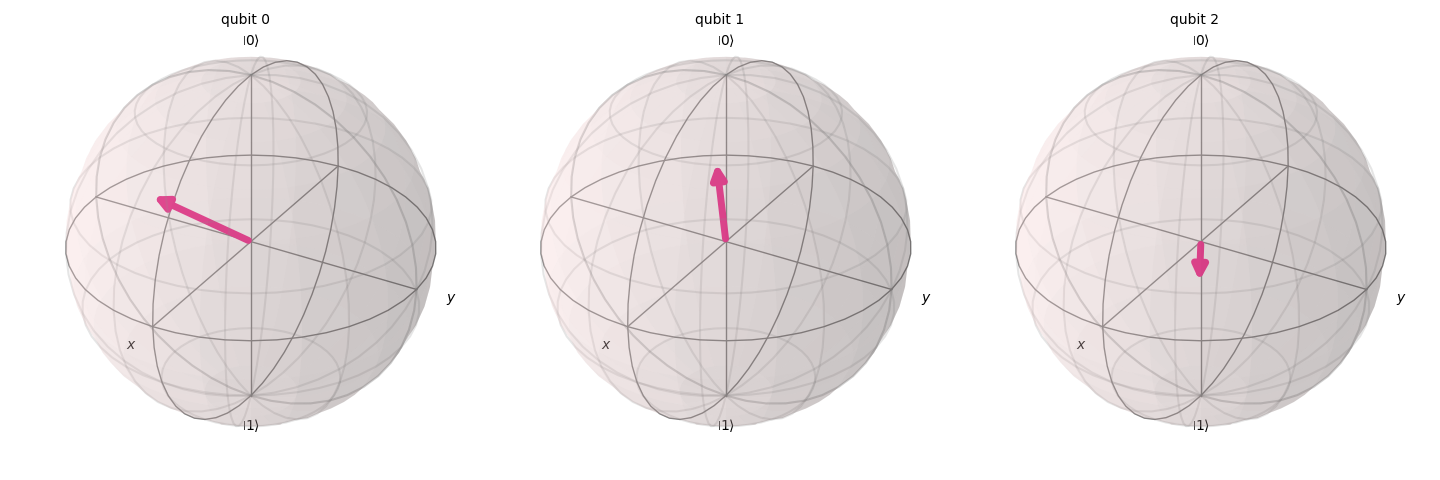
\includegraphics[width=\textwidth]{../QPCA-master/bloch_4x4.png}
            \captionof{figure}{Multivektor Bloch 4x4}
        \end{column}
        \begin{column}{0.5\textwidth}
            \small
            \begin{itemize}
                \item \textbf{Kontraksi Vektor:} Pemendekan panjang vektor ($r < 1$) mengindikasikan transisi dari \textit{pure state} menuju \textit{mixed state}.
                \item \textbf{Disorientasi Fase:} Akumulasi fase parasit merusak akurasi kalkulasi spektral finansial akibat noise sistemik.
            \end{itemize}
        \end{column}
    \end{columns}
\end{frame}


\end{document}
